\documentclass[10pt,a4paper,twoside]{article}

% ============================================================================
% A4 ACADEMIC MANUSCRIPT LAYOUT
% Wider, readable A4 text block with Times-style typography and monochrome tables
% ============================================================================
\usepackage[utf8]{inputenc}
\usepackage[T1]{fontenc}
\usepackage{newtxtext,newtxmath} % Springer Times New Roman text & math font
\usepackage[a4paper,left=20mm,right=20mm,top=12mm,bottom=18mm]{geometry}
\usepackage{microtype}           % Improved character protrusion and spacing
\usepackage{ragged2e}            % Explicit full paragraph justification
\usepackage{amsmath,amsfonts}
\usepackage{booktabs}            % Monochrome academic tables (\toprule, \midrule, \bottomrule)
\usepackage{tabularx}
\usepackage{array}
\usepackage{graphicx}
\graphicspath{{figures/}}
\usepackage{caption}
\usepackage{fancyhdr}
\usepackage{titlesec}
\usepackage{cite}                % Sequential numeric bracketed citations [1]-[27]
\usepackage[hidelinks]{hyperref} % Uniform black links with zero color boxes

% --- Springer Caption & Table Styling (Monochrome, Justified) ---
\captionsetup[figure]{font=footnotesize,labelfont=bf,labelsep=space,justification=justified,singlelinecheck=false,name=Fig.}
\captionsetup[table]{font=footnotesize,labelfont=bf,labelsep=space,justification=justified,singlelinecheck=false,name=Table}

% --- Springer Section Heading Typography ---
\titleformat{\section}{\normalfont\large\bfseries}{\thesection}{1em}{}
\titleformat{\subsection}{\normalfont\normalsize\bfseries}{\thesubsection}{1em}{}
\titleformat{\subsubsection}{\normalfont\normalsize\itshape}{\thesubsubsection}{1em}{}
\titlespacing*{\section}{0pt}{12pt plus 2pt minus 2pt}{5pt plus 1pt}
\titlespacing*{\subsection}{0pt}{9pt plus 2pt minus 1pt}{4pt plus 1pt}
\titlespacing*{\subsubsection}{0pt}{7pt plus 1pt minus 1pt}{3pt}

\setlength{\parindent}{1em}
\setlength{\parskip}{2pt}
\setlength{\emergencystretch}{2em}
\raggedbottom
\linespread{1.05}

% --- No running headers or footers ---
\pagestyle{empty}

\begin{document}
\justifying % Apply full justification to manuscript prose

% ============================================================================
% PAGE 1: TITLE, AUTHORS, ABSTRACT, KEYWORDS, & SECTION 1 START
% ============================================================================
\thispagestyle{empty}

\noindent{\small\textbf{Chapter 1}}\\[4pt]
{\LARGE\bfseries\raggedright InfraNova AI: Cross-Modal Translation of Thermal Infrared Satellite Imagery to Optical RGB Imagery Using a Residual Generative Framework\par}
\vspace{10pt}
\noindent{\normalsize\bfseries Soham Deshpande, Atharva Lingayat, Lokesh Gakhre, and Sanchit Wakde\par}\vspace{14pt}

\noindent\textbf{Abstract}\hspace{4pt}
Spaceborne thermal infrared (TIR) sensors, such as the Thermal Infrared Sensor 2 (TIRS-2) aboard Landsat 9, capture emitted longwave terrestrial radiation across both daytime and nighttime orbital passes independent of solar illumination. Although essential for surface energy balance modeling and nocturnal Earth observation, raw thermal captures are low-resolution scalar energy fields that lack visible color and high-frequency optical texture. Consequently, human analysts face significant difficulty interpreting complex land-cover topologies from raw thermal rasters, and pretrained optical computer vision models experience severe domain collapse due to contrast polarity inversions and diffuse structural edges. Mapping emitted thermal radiance ($10.6\text{--}12.5\,\mu\text{m}$) to visible optical reflectance ($0.45\text{--}0.67\,\mu\text{m}$) constitutes an ill-posed, many-to-one physical inverse problem: surface materials with nearly identical thermal inertia and kinetic temperature frequently exhibit vastly different optical albedos. Standard conditional Generative Adversarial Networks (cGANs) built on symmetrical U-Net backbones struggle in this cross-spectral regime. Their full-resolution skip connections channel raw, low-frequency thermal brightness gradients directly into the final decoding layers, inducing chromatic collapse, boundary ringing, and harsh magenta halos. In this paper, we present InfraNova AI, a cross-modal residual generative framework engineered for split-window thermal-to-optical satellite translation. By ingesting co-registered Landsat 9 TIRS-2 Band 10 and Band 11 rasters under independent local percentile normalization, our input pipeline preserves the atmospheric water-vapor and emissivity differential ($\Delta T = T_{10} - T_{11}$). Architecturally, we replace the skip-connected U-Net with a compact 11.37M-parameter Global ResNet Generator that routes representations through nine latent residual blocks at a $32 \times 32 \times 256$ bottleneck, cutting parameter overhead by 46.83\% while eliminating thermal gradient leakage. Furthermore, we identify and resolve an analytical backward-pass gradient singularity in perceptual color spaces by deriving a numerically stabilized CIE $L^*a^*b^*$ Euclidean chroma objective ($\varepsilon = 10^{-6}$) paired with a two-scale Spectral-Normalized Least-Squares GAN (LSGAN) discriminator. Evaluated across 1,259 geographically isolated test scenes, InfraNova AI improves Structural Similarity (SSIM) by +38.3\% (0.3254 to 0.4502), increases Peak Signal-to-Noise Ratio (PSNR) by +17.3\% (11.714 dB to 13.745 dB), reduces perceptual color error ($\Delta E^*_{ab}$) by 17.1\%, and yields a +42.1\% surge in downstream zero-shot YOLOv8 object detection recall.

\vspace{6pt}
\noindent\textbf{Keywords}\hspace{4pt} Cross-Modal Image Translation $\cdot$ Split-Window Thermal Infrared $\cdot$ Landsat 9 TIRS-2 $\cdot$ Conditional Generative Adversarial Networks $\cdot$ Global ResNet $\cdot$ LSGAN $\cdot$ CIE $L^*a^*b^*$ Chroma Regularization $\cdot$ Whole-Raster Inference

\section{Introduction}
Spaceborne Earth Observation (EO) operates across two physically distinct radiative regimes: the solar reflective spectrum ($0.4\text{--}2.5\,\mu\text{m}$) and the terrestrial thermal emissive spectrum ($8.0\text{--}14.0\,\mu\text{m}$) \cite{ref1}. Multispectral optical sensors, exemplified by the Operational Land Imager 2 (OLI-2) aboard Landsat 9, record solar electromagnetic radiation reflected from terrestrial surfaces at a $30\,\text{m}$ Ground Sample Distance (GSD) \cite{ref2}. While optical bands provide rich tristimulus color discrimination and crisp spatial edges, their utility is strictly bounded by solar geometry and atmospheric transparency---rendering optical sensors blind during nighttime orbital passes and over smoke- or haze-obscured terrain. Conversely, spaceborne thermal infrared (TIR) instruments, such as the Thermal Infrared Sensor 2 (TIRS-2) on Landsat 9, measure longwave radiation emitted directly by the Earth's surface across split-window channels Band 10 ($10.60\text{--}11.19\,\mu\text{m}$) and Band 11 ($11.50\text{--}12.51\,\mu\text{m}$) at a nominal $100\,\text{m}$ GSD \cite{ref2}. Because thermal emission is governed by subsurface heat flux and material thermodynamics rather than incident sunlight, TIRS-2 provides continuous round-the-clock observation critical for tracking urban heat islands, geothermal anomalies, nocturnal maritime corridors, industrial thermal plumes, and agricultural evapotranspiration stress \cite{ref3}.

% ============================================================================
% PAGE 2: SECTION 1 CONT. (PHYSICAL INVERSE PROBLEM, FIGURE 1, CONTRIBUTIONS)
% ============================================================================
Despite this operational resilience, deploying raw spaceborne thermal imagery within modern photogrammetric and computer vision workflows exposes three fundamental bottlenecks:

\begin{enumerate}
    \item \textbf{The Visual and Interpretive Barrier:} Raw thermal captures are single- or dual-channel scalar energy fields representing brightness temperature or top-of-atmosphere radiance. Human photo-interpreters rely heavily on chromatic hue, saturation, and high-frequency optical texture to segment complex landscapes. In monochrome thermal imagery, structurally distinct land-cover classes---such as dry fallow farmland, suburban concrete aprons, and exposed riverine silt---frequently share overlapping daytime or nighttime kinetic temperatures, appearing as indistinguishable gray intensities.
    \item \textbf{Downstream Vision Failure:} Modern automated geospatial intelligence pipelines rely on convolutional object detectors such as YOLOv8 \cite{ref4}, which are pretrained on millions of natural optical RGB images. When applied directly to raw thermal rasters, these detectors suffer complete domain collapse. This failure stems from both radiative thermal diffusion, which blurs sharp object boundaries across $100\,\text{m}$ sensor footprints, and contrast polarity inversions. Owing to the high specific heat capacity and thermal inertia of water relative to soil, rivers and coastal harbors appear thermally cold (pitch-black) during daytime solar heating, whereas at night they retain heat and appear bright white against rapidly cooling terrestrial backgrounds---inverting the edge gradients expected by optical feature extractors.
    \item \textbf{The Ill-Posed Physical Inverse Problem:} Translating emitted longwave thermal radiance into visible optical surface reflectance requires inverting two physically decoupled radiative transfer equations \cite{ref5}. In the thermal infrared window ($\lambda_t \in [10.6, 12.5]\,\mu\text{m}$), surface-leaving spectral radiance $L(\lambda_t, T_s)$ is governed by Planck's blackbody radiation law modulated by directional spectral emissivity $\varepsilon(\lambda_t)$ and surface kinetic temperature $T_s$:
\end{enumerate}

\begin{equation}
    \begin{aligned}
        L(\lambda_t,T_s)
        &= \varepsilon(\lambda_t)B(\lambda_t,T_s)
        + [1-\varepsilon(\lambda_t)]L_{\mathrm{atm}}^{\downarrow},\\
        B(\lambda_t,T_s)
        &= \frac{2hc^2}{\lambda_t^5\left[\exp\!\left(\frac{hc}{\lambda_t k_B T_s}\right)-1\right]}.
    \end{aligned}
    \label{eq:planck}
\end{equation}

where $h = 6.626 \times 10^{-34}\,\text{J}\cdot\text{s}$ denotes Planck's constant, $c = 2.998 \times 10^8\,\text{m/s}$ is the speed of light in vacuum, $k_B = 1.381 \times 10^{-23}\,\text{J/K}$ is the Boltzmann constant, and $L_{\mathrm{atm}}^{\downarrow}$ represents downwelling atmospheric thermal radiance reflected by the surface. In contrast, within the visible optical spectrum, represented here by red, green, and blue channels centered near $0.65\,\mu\text{m}$, $0.56\,\mu\text{m}$, and $0.48\,\mu\text{m}$, respectively, top-of-canopy surface reflectance $\rho(\lambda_v)$ is a dimensionless ratio governed by incident exoatmospheric solar irradiance $E_0(\lambda_v)$, solar zenith angle $\theta_s$, Earth-Sun astronomical distance $d$, and upward reflected optical radiance $L_{\mathrm{vis}}(\lambda_v)$:

\begin{equation}
    \rho(\lambda_v) = \frac{\pi \cdot L_{\mathrm{vis}}(\lambda_v) \cdot d^2}{E_0(\lambda_v) \cos\theta_s}
    \label{eq:reflectance}
\end{equation}

Because kinetic temperature $T_s$ is a bulk thermodynamic state governed by diurnal heat balance and thermal inertia $P = \sqrt{\kappa \rho_m c_p}$ (where $\kappa$ is thermal conductivity, $\rho_m$ is bulk density, and $c_p$ is specific heat capacity), whereas optical albedo $\rho(\lambda_v)$ is determined by molecular electronic transitions and chlorophyll/mineral pigment absorption in the uppermost micrometers of the surface, the inverse mapping $\mathcal{F}: (L_{10}, L_{11}) \mapsto (\rho_R, \rho_G, \rho_B)$ is inherently ill-posed and many-to-one.

\begin{figure}[htbp]
    \centering
    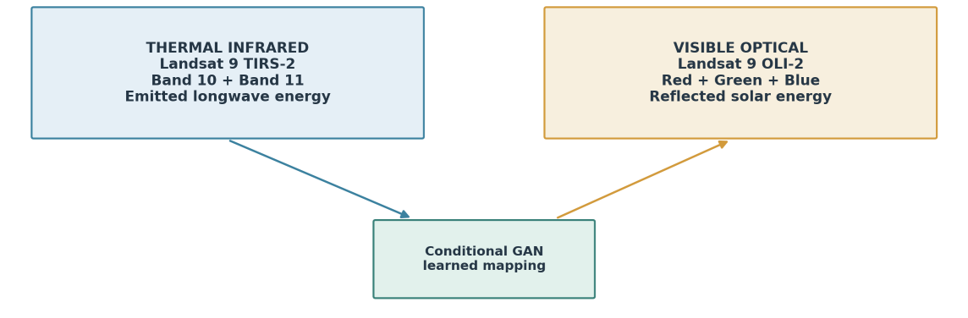
\includegraphics[width=\textwidth,height=0.42\textheight,keepaspectratio]{figures/fig1_cross_modal_modalities.png}
    \caption{Physical separation between emitted longwave thermal radiance (TIRS-2) and reflected solar optical irradiance (OLI-2).}
    \label{fig:decoupling}
\end{figure}

Standard cGANs \cite{ref6} fail in this regime due to chromatic collapse toward $\mathbb{E}[\mathbf{y} \mid \mathbf{x}]$ \cite{ref7} and U-Net skip-connection gradient leakage \cite{ref8, ref9, ref10}. The key contributions of this study are: (1) a dual-band split-window formulation preserving $\Delta T = T_{10} - T_{11}$; (2) a skip-free 11.37M-parameter Global ResNet Generator cutting parameters by 46.83\%; (3) an $\varepsilon$-stabilized CIE $L^*a^*b^*$ chroma loss ($\varepsilon = 10^{-6}$) bounding backward derivatives to $\le 500.0$; and (4) comprehensive validation across 1,259 unseen scenes showing +38.3\% SSIM, +17.3\% PSNR, and +42.1\% YOLOv8n recall.

The organization of the paper is as follows: Sect.~2 reviews related work. Section~3 presents the proposed methodology. Section~4 discusses experimental ablations, downstream YOLOv8 validation, and whole-raster tiling, and Sect.~5 concludes the paper.

% ============================================================================
% PAGE 3: SECTION 2 (RELATED WORK: 2.1 & 2.2)
% ============================================================================
\section{Related Work}

\subsection{Generative Adversarial Networks and Image-to-Image Translation}
Conditional Generative Adversarial Networks (cGANs) were established as a unified framework for paired image-to-image translation by Isola et al.~\cite{ref6} in Pix2Pix. By conditioning both an encoder-decoder generator $G$ and a Markovian PatchGAN discriminator $D$ \cite{ref11} on a source spatial raster $\mathbf{x}$, Pix2Pix optimizes a minimax game jointly with a pixel-wise $L_1$ reconstruction objective. To scale conditional synthesis to higher resolutions and stabilize adversarial dynamics, Wang et al.~\cite{ref8} introduced Pix2PixHD, which replaced the single-scale discriminator with a multi-scale PatchGAN hierarchy evaluating image pyramids at multiple receptive fields, introduced a discriminator feature-matching loss, and utilized a residual global generator backbone \cite{ref12}. Concurrently, Mao et al.~\cite{ref13} demonstrated in Least-Squares GAN (LSGAN) that replacing the standard sigmoid Binary Cross-Entropy (BCE) discriminator loss with a quadratic least-squares penalty prevents vanishing gradients when synthesized samples lie on the correct side of the decision boundary but remain far from the true data manifold. In unpaired translation scenarios where co-registered ground truth is unavailable, Zhu et al.~\cite{ref14} proposed CycleGAN, enforcing cycle-consistency constraints $F(G(\mathbf{x})) \approx \mathbf{x}$ across domains.

While these foundational architectures achieve strong performance in paired visible-to-visible or structurally isomorphic translation---where spatial edges in the input match 1:1 with luminance boundaries in the output---their architectural inductive biases break down in cross-modal, cross-spectral satellite translation. In intra-modal tasks (such as optical super-resolution or semantic label-to-photo synthesis), skip connections in a U-Net \cite{ref6, ref9} beneficially transfer high-frequency spatial phase information directly across the network bottleneck. In spaceborne thermal-to-optical translation, however, the input measures emitted $100\,\text{m}$ thermal radiation whereas the target measures reflected $30\,\text{m}$ solar irradiance. Edge polarities frequently invert between diurnal passes, and sharp optical boundaries (such as road networks and field borders) are thermally diffused. Retaining U-Net skip connections in this cross-spectral regime provides a detrimental shortcut: the generator bypasses semantic abstraction in the bottleneck and leaks raw, low-frequency thermal brightness gradients directly into the final RGB convolutions, resulting in severe boundary ringing and magenta coastal halos. Furthermore, because Landsat 9 captures TIRS-2 and OLI-2 swaths simultaneously from the same orbital platform, unpaired CycleGAN formulations are counterproductive, as they discard exact pixel-level ground-truth registration and introduce geometric hallucinations.

\subsection{Thermal Infrared Colorization}
Early approaches to visualizing single-band thermal imagery relied on deterministic pseudo-coloring Look-Up Tables (LUTs)---such as Ironbow, Rainbow, or Inferno colormaps---or linear intensity-hue-saturation (IHS) fusion with panchromatic channels \cite{ref1}. Although pseudo-color LUTs assist human operators in spotting relative temperature extrema, the resulting false colors bear no physical correlation to true optical surface reflectance, causing pretrained optical object detectors to fail completely.

With the rise of convolutional neural networks, Berg et al.~\cite{ref15} and Nyberg et al.~\cite{ref16} investigated deep autoencoders and adversarial networks to colorize single-band forward-looking infrared (FLIR) imagery for automotive nighttime pedestrian detection. Kuang et al.~\cite{ref17} extended this framework using a coarse-to-fine conditional GAN on terrestrial surveillance datasets, while Luo et al.~\cite{ref18} incorporated object-appearance feedback for low-altitude unmanned aerial vehicle (UAV) thermal video.

However, existing thermal colorization literature exhibits three major limitations when applied to spaceborne Earth Observation:
\begin{enumerate}
    \item \textbf{Single-Band Airborne/Ground Scope vs.~Planetary Diversity:} Prior studies predominantly address single-band broadband thermal video ($8\text{--}14\,\mu\text{m}$) captured at close range ($10\text{--}100\,\text{m}$) over small, homogeneous urban streetscapes rather than nadir spaceborne satellite imagery at $100\,\text{m}$ GSD spanning diverse global biomes (deserts, alpine cryospheres, tropical rainforests, coastal waters, and megacities).
    \item \textbf{Neglect of Split-Window Radiometric Physics:} Existing deep learning pipelines ingest a single thermal band as a grayscale image. In spaceborne radiometry, a single thermal channel cannot separate surface kinetic temperature from atmospheric water-vapor attenuation and material emissivity variations \cite{ref3, ref5}. Formulating spaceborne translation using dual-band split-window channels (Landsat 9 Bands 10 and 11) with independent local contrast normalization to preserve the physical differential $\Delta T = T_{10} - T_{11}$ has remained unaddressed.
    \item \textbf{Lack of Downstream Photogrammetric Verification:} Prior remote sensing translation studies evaluate outputs almost exclusively via pixel distortion metrics (PSNR and SSIM), without testing whether the synthesized optical rasters restore zero-shot object detection recall in operational detectors such as YOLOv8 \cite{ref4}.
\end{enumerate}

% ============================================================================
% PAGE 4: SECTION 2.3 & SECTION 3.1 (DATASET ACQUISITION, FIGURE 2)
% ============================================================================
\subsection{Perceptual and Color Regularization Schemes}
Because pixel-wise $L_1$ and $L_2$ objectives average over uncertain color modes \cite{ref7}, conditional GANs commonly incorporate VGG Perceptual Loss \cite{ref19, ref20} and discriminator Feature Matching Loss \cite{ref8}. While VGG perceptual supervision improves structural edge coherence, classification networks trained on ImageNet are optimized for invariance to illumination and color tint; consequently, VGG feature loss alone does not prevent systematic chromatic desaturation. Heuristic RGB color variance losses attempt to combat desaturation by penalizing differences in the standard deviation of Red, Green, and Blue channels at each pixel. However, because luminance and chrominance are entangled in the RGB color cube, penalizing RGB channel variance inadvertently penalizes legitimate luminance shading gradients instead of pure chroma magnitude, leading to acute desaturation across agricultural landscapes when tuned aggressively. Formulating saturation supervision in the perceptual CIE $L^*a^*b^*$ color space orthogonalizes lightness ($L^*$) from opponent color channels ($a^*, b^*$), but requires analytical stabilization of the Euclidean chroma square-root derivative at achromatic pixels.

\section{Proposed Methodology}

\subsection{Dataset Acquisition, Filtering, and Geographic Splitting}
We engineered an automated acquisition and preprocessing pipeline interfacing with the \textbf{Landsat 9 Collection 2 Level-2} science archive via Google Earth Engine (GEE) \cite{ref2, ref21}. Each acquired scene comprises co-registered, simultaneously captured observations from two onboard instruments:
\begin{itemize}
    \item \textbf{Split-Window Thermal Infrared Input ($\mathbf{x} \in \mathbb{R}^{2 \times H \times W}$):} Level-2 Surface Temperature (ST) products from TIRS-2, comprising \textbf{Band 10} ($10.60\text{--}11.19\,\mu\text{m}$) and \textbf{Band 11} ($11.50\text{--}12.51\,\mu\text{m}$) at a native $100\,\text{m}$ GSD, stored as continuous 32-bit IEEE-754 floating-point arrays (\texttt{.npy}).
    \item \textbf{Visible Optical Reflectance Target ($\mathbf{y} \in \mathbb{R}^{3 \times H \times W}$):} Level-2 Surface Reflectance (SR) products from OLI-2, comprising \textbf{Band 4} (Red, $0.64\text{--}0.67\,\mu\text{m}$), \textbf{Band 3} (Green, $0.53\text{--}0.59\,\mu\text{m}$), and \textbf{Band 2} (Blue, $0.45\text{--}0.51\,\mu\text{m}$) at a native $30\,\text{m}$ GSD.
\end{itemize}

\subsubsection{Spatial Resampling and Patch Quality Control}
Because OLI-2 captures visible reflectance at $30\,\text{m}$ GSD whereas TIRS-2 resolves thermal emission at $100\,\text{m}$ GSD, direct pixel-to-pixel supervision requires spatial co-registration onto a common grid. Upsampling $100\,\text{m}$ thermal bands to $30\,\text{m}$ fabricates synthetic interpolated frequencies not measured by the thermal sensor. Instead, we downsample the $30\,\text{m}$ RGB channels to the exact $100\,\text{m}$ thermal lattice using \textbf{area-averaging decimation} (\texttt{cv2.INTER\_AREA}), which integrates optical photons across each $100\,\text{m} \times 100\,\text{m}$ ground cell and prevents spatial aliasing.

From the co-registered $100\,\text{m}$ scenes, \textbf{66,780 multi-spectral patch pairs} are extracted at $128 \times 128$ resolution ($12.8\,\text{km} \times 12.8\,\text{km}$ ground footprint per patch) using a sliding window stride of 32 pixels (75\% spatial overlap). To eliminate orbital swath borders, sensor drop-outs, and thick convective cloud masks, an automated quality-control filter inspects every candidate patch: any patch with $>50\%$ unpopulated/zero pixels, zero spatial variance, or containing non-finite values (\texttt{NaN} or \texttt{Inf}) in either thermal or optical channels is automatically quarantined and discarded.

\begin{figure}[htbp]
    \centering
    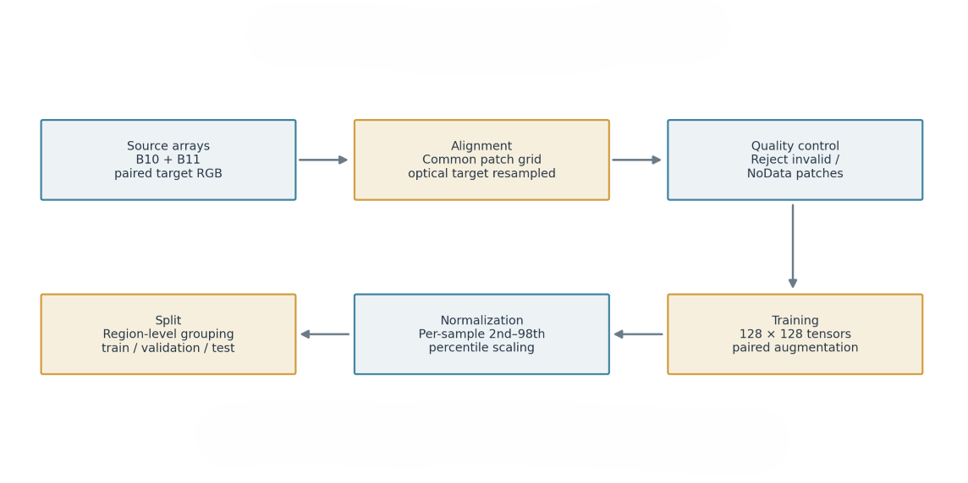
\includegraphics[width=\textwidth,height=0.42\textheight,keepaspectratio]{figures/fig2_data_preparation_workflow.png}
    \caption{End-to-End Data Pipeline Flowchart showing Landsat 9 scene acquisition $\to$ area resampling ($30\,\text{m} \to 100\,\text{m}$) $\to$ sliding window extraction ($128 \times 128$, stride 32) $\to$ NaN/zero filtering $\to$ geographic non-leakage splitting $\to$ local percentile normalization.}
    \label{fig:pipeline}
\end{figure}

% ============================================================================
% PAGE 5: SECTION 3.1 CONT. (SPLITTING, EQ. 3, TABLE 1) & SECTION 3.2 (EQ. 4)
% ============================================================================
\subsubsection{Geographic Partitioning (Zero-Leakage Protocol)}
Because patches extracted with a 32-pixel stride overlap by 75\% spatially, random patch-level splitting places overlapping views of the exact same cities, rivers, and agricultural parcels into both training and test sets, causing severe spatial autocorrelation leakage. To guarantee zero spatial leakage, dataset partitioning is executed strictly at the WRS-2 scene path/row geographic footprint level, as summarized in Table~\ref{tab:dataset}. Patches from the same geographic region never appear across splits.

\begin{table}[htbp]
    \caption{Dataset distribution, geographic split protocol, and spatial support.}
    \label{tab:dataset}
    \centering
    \footnotesize
    \begin{tabularx}{\textwidth}{@{}>{\raggedright\arraybackslash}p{1.55cm}>{\centering\arraybackslash}p{2.0cm}>{\centering\arraybackslash}p{1.1cm}>{\raggedright\arraybackslash}X@{}}
        \toprule
        \textbf{Dataset split} & \textbf{Active tiles} & \textbf{Share} & \textbf{Spatial support and integrity control} \\
        \midrule
        Training & 10,565 (53,424 full corpus) & 80\% & $128 \times 128$ at $100\,\text{m}$ GSD ($12.8 \times 12.8\,\text{km}$). \\
        Validation & 1,432 & 10\% & Geographically isolated WRS-2 path/row scenes. \\
        Held-out test & 1,259 & 10\% & SHA-256 locked (\texttt{894cfcd2ae764ff0c43ff3fa...}). \\
        \midrule
        \textbf{Total} & \textbf{13,256 (66,780 extracted)} & \textbf{100\%} & \textbf{No spatial overlap across splits.} \\
        \bottomrule
    \end{tabularx}
\end{table}

\subsubsection{Local Percentile Contrast Normalization}
Absolute surface temperatures vary by over $80\,\text{K}$ across global biomes. Applying fixed global normalization crushes local thermal contrast within individual scenes, whereas normalizing Band 10 and Band 11 jointly with a shared scalar erases the inter-band split-window calibration offset. For each patch $\mathbf{x}$ and each thermal band $c \in \{\text{Band 10}, \text{Band 11}\}$, we apply independent 2nd--98th percentile scaling into $[-1, 1]$:

\begin{equation}
    \tilde{\mathbf{x}}_c = 2 \cdot \operatorname{clip}\!\left( \frac{\mathbf{x}_c - P_2(\mathbf{x}_c)}{P_{98}(\mathbf{x}_c) - P_2(\mathbf{x}_c) + 10^{-8}}, \, 0, \, 1 \right) - 1, \quad \text{for } c \in \{\text{Band 10}, \text{Band 11}\}
    \label{eq:percentile}
\end{equation}

where $P_2(\mathbf{x}_c)$ and $P_{98}(\mathbf{x}_c)$ denote the local 2nd and 98th percentiles of band $c$, and $10^{-8}$ prevents division by zero on isothermal water patches. Normalizing Band 10 and Band 11 independently maximizes local structural contrast while preserving the split-window radiance differential $\Delta T = T_{10} - T_{11}$. During training, paired data augmentations include horizontal flips ($p = 0.5$), vertical flips ($p = 0.5$), orthogonal $90^\circ$ rotations, and $\pm 10\%$ brightness/contrast jitter.

\subsection{Network Architecture: Global ResNet Generator}
To prevent raw thermal brightness gradients from leaking across encoder-decoder skip connections, we replace the U-Net with a skip-free \textbf{Global ResNet Generator} (\texttt{Pix2PixHDGlobalResNetGenerator}, 11,369,795 trainable parameters) \cite{ref8, ref12, ref19}. Given a normalized 2-channel input tensor $\tilde{\mathbf{x}} \in \mathbb{R}^{B \times 2 \times 128 \times 128}$, the network executes sequentially across four stages:

\begin{enumerate}
    \item \textbf{Initial Stem (Layer 1):} \texttt{ReflectionPad2d(3)} (mirroring boundary pixels to eliminate zero-padding border artifacts) $\to$ \texttt{Conv2d(2, 64, kernel=7, stride=1, bias=False)} $\to$ \texttt{InstanceNorm2d(64)} \cite{ref22} $\to$ \texttt{ReLU}, yielding $[B, 64, 128, 128]$.
    \item \textbf{Strided Downsampling Stages:}
          \begin{itemize}
              \item \textit{Downsampling 1:} a $3 \times 3$ convolution maps 64 to 128 channels with stride 2 and padding 1, followed by InstanceNorm and ReLU. The output is $[B,128,64,64]$.
              \item \textit{Downsampling 2:} a second $3 \times 3$ convolution maps 128 to 256 channels with stride 2 and padding 1, followed by InstanceNorm and ReLU. The output is $[B,256,32,32]$.
          \end{itemize}
    \item \textbf{Latent Residual Bottleneck (9 ResNet Blocks):} Rather than collapsing spatial dimensions to $1 \times 1$, the architecture halts downsampling at $32 \times 32$ and routes the latent representation $\mathbf{z}_0 \in \mathbb{R}^{B \times 256 \times 32 \times 32}$ through \textbf{9 consecutive ResNet blocks}. Each residual block $l \in \{1, \dots, 9\}$ computes:
\end{enumerate}

\begin{equation}
    \mathbf{z}_l = \mathbf{z}_{l-1} + \left[ \operatorname{IN} \circ \operatorname{Conv}_{3\times 3} \circ \operatorname{Pad}_1 \circ \operatorname{ReLU} \circ \operatorname{IN} \circ \operatorname{Conv}_{3\times 3} \circ \operatorname{Pad}_1 \right](\mathbf{z}_{l-1})
    \label{eq:resnet}
\end{equation}

where $\operatorname{Pad}_1$ denotes one-pixel reflection padding, $\operatorname{Conv}_{3\times 3}$ denotes a $3 \times 3$ convolution that preserves 256 channels, and $\operatorname{IN}$ denotes Instance Normalization over those channels.

% ============================================================================
% PAGE 6: SECTION 3.2 CONT., FIGURE 3, & TABLE 2 (ARCHITECTURE BREAKDOWN)
% ============================================================================
\begin{enumerate}
    \setcounter{enumi}{3}
    \item \textbf{Transposed-Convolutional Upsampling and Output Head:}
          \begin{itemize}
              \item \textit{Upsampling 1:} a $3 \times 3$ transposed convolution maps 256 to 128 channels and doubles the spatial dimensions. InstanceNorm and ReLU follow; output: $[B,128,64,64]$.
              \item \textit{Upsampling 2:} a second transposed convolution maps 128 to 64 channels and restores $128 \times 128$ resolution. InstanceNorm and ReLU follow; output: $[B,64,128,128]$.
              \item \textit{Output layer:} reflection padding and a $7 \times 7$ convolution produce three RGB channels, followed by Tanh; output: $\hat{\mathbf{y}} \in [-1,1]^{B \times 3 \times 128 \times 128}$.
          \end{itemize}
\end{enumerate}

\begin{figure}[htbp]
    \centering
    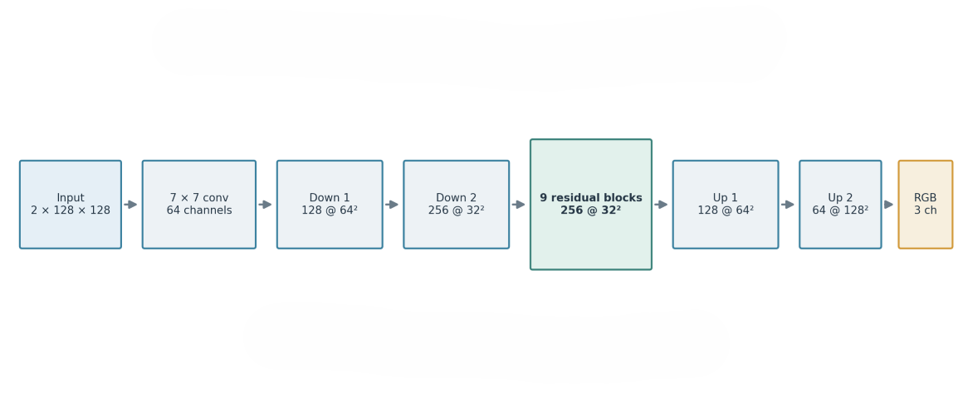
\includegraphics[width=\textwidth,height=0.42\textheight,keepaspectratio]{figures/fig3_exp9_global_resnet_generator.png}
    \caption{Global ResNet Generator Architecture (11.37M Parameters) showing input convolution $\to$ 2 downsampling stages $\to$ 9 residual blocks at $32 \times 32 \times 256$ bottleneck $\to$ 2 transposed conv upsampling stages $\to$ final $7 \times 7$ output projection with $\tanh$.}
    \label{fig:generator}
\end{figure}

\begin{table}[htbp]
    \caption{Layer-by-layer architectural specification and parameter breakdown of the Global ResNet Generator versus the Legacy U-Net Baseline.}
    \label{tab:arch}
    \centering
    \scriptsize
    \setlength{\tabcolsep}{3.8pt}
    \begin{tabularx}{\textwidth}{@{}>{\raggedright\arraybackslash}p{1.55cm}>{\raggedright\arraybackslash}X>{\centering\arraybackslash}p{2.05cm}>{\raggedleft\arraybackslash}p{1.2cm}@{}}
        \toprule
        \textbf{Stage} & \textbf{Operation, normalization and activation} & \textbf{Output shape} & \textbf{Params.} \\
        \midrule
        Input stem & Reflection padding; $7 \times 7$ convolution (2 to 64 channels); InstanceNorm; ReLU. & $[B,64,128,128]$ & 6,400 \\
        Downsample 1 & $3 \times 3$ convolution, stride 2 (64 to 128 channels); InstanceNorm; ReLU. & $[B,128,64,64]$ & 73,984 \\
        Downsample 2 & $3 \times 3$ convolution, stride 2 (128 to 256 channels); InstanceNorm; ReLU. & $[B,256,32,32]$ & 295,424 \\
        Bottleneck & Nine residual blocks, each with two $3 \times 3$ convolutions at 256 channels, reflection padding, InstanceNorm and ReLU. & $[B,256,32,32]$ & 10,626,048 \\
        Upsample 1 & Transposed convolution (256 to 128 channels), stride 2; InstanceNorm; ReLU. & $[B,128,64,64]$ & 295,168 \\
        Upsample 2 & Transposed convolution (128 to 64 channels), stride 2; InstanceNorm; ReLU. & $[B,64,128,128]$ & 73,856 \\
        Output & Reflection padding; $7 \times 7$ convolution (64 to 3 channels); Tanh. & $[B,3,128,128]$ & 9,411 \\
        \midrule
        \textbf{Proposed total} & \textbf{Skip-free Global ResNet Generator} & $[B,3,128,128]$ & \textbf{11,369,795} \\
        Legacy baseline & Symmetrical skip-connected U-Net; InstanceNorm and LeakyReLU/ReLU. & $[B,3,128,128]$ & 21,383,238 \\
        \bottomrule
    \end{tabularx}
\end{table}

\noindent\textbf{Physical Justification of Skip-Connection Removal:} As detailed in Table~\ref{tab:arch}, the 9 residual blocks at the $32 \times 32 \times 256$ bottleneck house 10,626,048 parameters (93.46\% of the generator's capacity). Removing symmetrical encoder-decoder skip connections forces all spatial and radiometric features to pass through the 18 convolutional layers of this latent bottleneck. Rather than tinting raw thermal brightness edges leaked from early encoding stages, the bottleneck aggregates wide-area geomorphological context (river meanders, road grids, agricultural parcel boundaries) and synthesizes true optical land-cover representations while cutting parameter count by \textbf{46.83\%} (saving 10,013,443 parameters).

% ============================================================================
% PAGE 7: SECTION 3.3 (DISCRIMINATOR, EQS. 5-6, FIGURE 4)
% ============================================================================
\subsection{Multi-Scale PatchGAN Discriminator and Spectral Normalization}
We employ a two-scale Markovian PatchGAN discriminator $D = (D_1, D_2)$ (5,532,418 parameters) conditioned on the 5-channel concatenation $\mathbf{u} = \operatorname{cat}(\tilde{\mathbf{x}}, \mathbf{y}) \in \mathbb{R}^{B \times 5 \times 128 \times 128}$. Fine scale $D_1$ operates at native $128 \times 128$ resolution, while coarse scale $D_2$ operates at $64 \times 64$ resolution via \texttt{AvgPool2d(kernel=3, stride=2, padding=1)}, with each branch enforcing a $70 \times 70$ receptive field across five $4 \times 4$ convolutional layers ($64 \to 128 \to 256 \to 512 \to 1$) with \texttt{LeakyReLU(0.2)}.

To enforce the 1-Lipschitz continuity bound ($\|D_k(\mathbf{u}_1) - D_k(\mathbf{u}_2)\|_2 \le \|\mathbf{u}_1 - \mathbf{u}_2\|_2$) and prevent discriminator gradient explosions during cross-modal training, Spectral Normalization \cite{ref23} is applied to every convolutional weight matrix $W_l$ via power iteration:

\begin{equation}
    \bar{W}_{\mathrm{SN}}(W_l) = \frac{W_l}{\sigma(W_l)}, \quad \text{where } \sigma(W_l) = \max_{\mathbf{h} \neq \mathbf{0}} \frac{\|W_l \mathbf{h}\|_2}{\|\mathbf{h}\|_2} \le 1
    \label{eq:sn}
\end{equation}

Crucially, \texttt{InstanceNorm2d} is explicitly omitted from all discriminator blocks. Because Instance Normalization rescales feature activations $\mathbf{h}$ dynamically by the inverse mini-batch spatial standard deviation $\gamma / \sqrt{\sigma^2(\mathbf{h}) + \varepsilon}$, homogeneous ocean or desert patches (where $\sigma^2(\mathbf{h}) \to 0$) amplify the effective singular value far above unity:

\begin{equation}
    \operatorname{IN}(\mathbf{h}) = \gamma \left( \frac{\mathbf{h} - \mu(\mathbf{h})}{\sqrt{\sigma^2(\mathbf{h}) + \varepsilon}} \right) + \beta \implies \sigma\!\left( \operatorname{diag}\!\left(\frac{\gamma}{\sqrt{\sigma^2(\mathbf{h}) + \varepsilon}}\right) \bar{W}_{\mathrm{SN}} \right) \gg 1
    \label{eq:in_violation}
\end{equation}

Omitting \texttt{InstanceNorm2d} and relying exclusively on Spectral Normalization strictly preserves the 1-Lipschitz bound across all training iterations.

\begin{figure}[htbp]
    \centering
    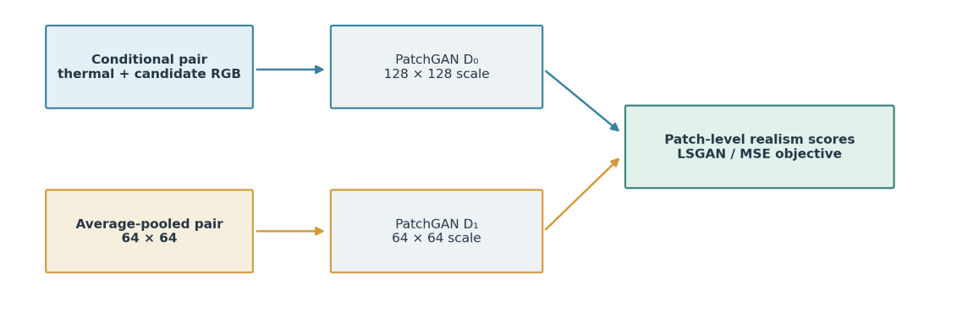
\includegraphics[width=\textwidth,height=0.42\textheight,keepaspectratio]{figures/fig4_two_scale_discriminator.png}
    \caption{Multi-Scale Discriminator \& Spectral Normalization Architecture showing $D_1$ and $D_2$ with Spectral Normalization and the absence of Instance Normalization to preserve the 1-Lipschitz bound.}
    \label{fig:discriminator}
\end{figure}

% ============================================================================
% PAGE 8: SECTION 3.4 (MULTI-TASK OBJECTIVE FUNCTION: EQS. 7-13)
% ============================================================================
\subsection{Multi-Task Objective Function Formulation}
The Global ResNet Generator is optimized under a six-term multi-task objective function:

\begin{equation}
    \mathcal{L}_{\mathrm{total}} = \lambda_{\mathrm{adv}}\mathcal{L}_{\mathrm{GAN}} + \lambda_{\mathrm{L1}}\mathcal{L}_{\mathrm{L1}} + \lambda_{\mathrm{perc}}\mathcal{L}_{\mathrm{perc}} + \lambda_{\mathrm{ssim}}\mathcal{L}_{\mathrm{ssim}} + \lambda_{\mathrm{chroma}}\mathcal{L}_{\mathrm{chroma}} + \lambda_{\mathrm{sat}}\mathcal{L}_{\mathrm{sat}}
    \label{eq:total_loss}
\end{equation}

with locked optimal weights $\lambda_{\mathrm{adv}} = 1.0$, $\lambda_{\mathrm{L1}} = 10.0$, $\lambda_{\mathrm{perc}} = 5.0$, $\lambda_{\mathrm{ssim}} = 5.0$, $\lambda_{\mathrm{chroma}} = 2.0$, $\lambda_{\mathrm{sat}} = 0.05$, and $\lambda_{\mathrm{feat}} = 0.0$.

\subsubsection{Multi-Scale Least-Squares Adversarial Objective (\texorpdfstring{$\mathcal{L}_D^{\mathrm{LSGAN}}, \mathcal{L}_G^{\mathrm{LSGAN}}$}{LSGAN discriminator and generator losses})}
To eliminate the early vanishing-gradient saturation of Binary Cross-Entropy (BCE), we employ a Least-Squares GAN (LSGAN) objective \cite{ref13} averaged across both discriminator scales $k \in \{1, 2\}$:

\begin{equation}
    \begin{aligned}
        \mathcal{L}_D^{\mathrm{LSGAN}} = \frac{1}{2}\sum_{k=1}^{2}\Big(&\mathbb{E}_{\mathbf{x},\mathbf{y}}[(D_k(\mathbf{x},\mathbf{y})-1)^2]\\
        &+\mathbb{E}_{\mathbf{x}}[D_k(\mathbf{x},G(\mathbf{x}))^2]\Big).
    \end{aligned}
    \label{eq:lsgan_d}
\end{equation}

\begin{equation}
    \mathcal{L}_G^{\mathrm{LSGAN}} = \frac{1}{2}\sum_{k=1}^{2} \mathbb{E}_{\mathbf{x}}\!\left[(D_k(\mathbf{x}, G(\mathbf{x})) - 1)^2\right]
    \label{eq:lsgan_g}
\end{equation}

\subsubsection{Pixel-Level \texorpdfstring{$L_1$}{L1} Reconstruction Loss (\texorpdfstring{$\mathcal{L}_{\mathrm{L1}}$}{L1 loss})}
Low-frequency radiometric intensity and broad tonal consistency are anchored by the pixel-wise $L_1$ distance:

\begin{equation}
    \mathcal{L}_{\mathrm{L1}}(\hat{\mathbf{y}}, \mathbf{y}) = \frac{1}{3HW}\|\hat{\mathbf{y}} - \mathbf{y}\|_1 = \frac{1}{3HW}\sum_{c=1}^{3}\sum_{u=1}^{H}\sum_{v=1}^{W} \left|\hat{y}_{c,u,v} - y_{c,u,v}\right|
    \label{eq:l1}
\end{equation}

\subsubsection{Differentiable Structural Similarity Loss (\texorpdfstring{$\mathcal{L}_{\mathrm{ssim}}$}{SSIM loss})}
To preserve local spatial contrast, road networks, and riverine boundaries, we incorporate a differentiable SSIM loss \cite{ref24} using an $11 \times 11$ Gaussian window ($C_1 = 0.01^2, C_2 = 0.03^2$):

\begin{equation}
    \begin{aligned}
        \mathcal{L}_{\mathrm{ssim}}(\hat{\mathbf{y}},\mathbf{y})
        &= \frac{1-\operatorname{SSIM}(\hat{\mathbf{y}},\mathbf{y})}{2},\\
        \operatorname{SSIM}(\hat{\mathbf{y}},\mathbf{y})
        &= \frac{(2\mu_{\hat{\mathbf{y}}}\mu_{\mathbf{y}}+C_1)
        (2\sigma_{\hat{\mathbf{y}}\mathbf{y}}+C_2)}
        {(\mu_{\hat{\mathbf{y}}}^{2}+\mu_{\mathbf{y}}^{2}+C_1)
        (\sigma_{\hat{\mathbf{y}}}^{2}+\sigma_{\mathbf{y}}^{2}+C_2)}.
    \end{aligned}
    \label{eq:ssim}
\end{equation}

\subsubsection{VGG-19 Perceptual and RGB Chroma Dispersion Losses (\texorpdfstring{$\mathcal{L}_{\mathrm{perc}}, \mathcal{L}_{\mathrm{chroma}}$}{perceptual and chroma losses})}
High-level semantic land-cover features are supervised across frozen VGG-19 \cite{ref19, ref20} feature layers $\mathcal{V} = \{\texttt{relu1\_2}, \texttt{relu2\_2}, \texttt{relu3\_4}, \texttt{relu4\_4}\}$, paired with a baseline per-pixel RGB standard-deviation dispersion penalty:

\begin{equation}
    \mathcal{L}_{\mathrm{perc}}(\hat{\mathbf{y}}, \mathbf{y}) = \sum_{l \in \mathcal{V}} \frac{1}{C_l H_l W_l}\left\|\phi_l(\hat{\mathbf{y}}) - \phi_l(\mathbf{y})\right\|_1
    \label{eq:perc}
\end{equation}

\begin{equation}
    \begin{aligned}
        \mathcal{L}_{\mathrm{chroma}}(\hat{\mathbf{y}},\mathbf{y})
        &= \frac{1}{HW}\sum_{u,v}
        \left|\sigma_{\mathrm{RGB}}(\hat{\mathbf{y}}_{u,v})
        -\sigma_{\mathrm{RGB}}(\mathbf{y}_{u,v})\right|,\\
        \sigma_{\mathrm{RGB}}(\mathbf{y}_{u,v})
        &= \sqrt{\frac{1}{3}\sum_{c\in\{R,G,B\}}
        (y_{c,u,v}-\bar y_{u,v})^2+10^{-6}}.
    \end{aligned}
    \label{eq:chroma}
\end{equation}

% ============================================================================
% PAGE 9: SECTION 3.4 CONT. (CIE LAB SINGULARITY DERIVATION, EQS. 14-18, FIG. 5) & 3.5
% ============================================================================
\subsubsection{Numerically Stabilized CIE \texorpdfstring{$L^*a^*b^*$}{Lab} Saturation Loss and Singularity Solution}
Because RGB channel dispersion $\sigma_{\mathrm{RGB}}$ entangles luminance with chrominance, tuning $\lambda_{\mathrm{chroma}}$ aggressively drains natural color from agricultural parcels (\texttt{Exp3}). To decouple lightness from chrominance, linear sRGB in $[0, 1]$ is projected to CIE XYZ (D65 white point: $X_n = 0.95047, Y_n = 1.00000, Z_n = 1.08883$) and transformed into CIE 1976 $L^*a^*b^*$ opponent coordinates ($L^*, a^*, b^*$) via the piecewise cube-root transfer function $f(t)$:

\begin{equation}
    \begin{aligned}
        L^* &= 116f\!\left(\frac{Y}{Y_n}\right)-16,\\
        a^* &= 500\left[f\!\left(\frac{X}{X_n}\right)
        -f\!\left(\frac{Y}{Y_n}\right)\right],\\
        b^* &= 200\left[f\!\left(\frac{Y}{Y_n}\right)
        -f\!\left(\frac{Z}{Z_n}\right)\right].
    \end{aligned}
    \label{eq:lab_coords}
\end{equation}

\begin{equation}
    f(t) = \begin{cases}
        t^{1/3}                                                 & \text{if } t > \left(\frac{6}{29}\right)^3 \approx 0.008856 \\
        \frac{1}{3}\left(\frac{29}{6}\right)^2 t + \frac{4}{29} & \text{otherwise}
    \end{cases}
    \label{eq:lab_transfer}
\end{equation}

In an unstabilized Euclidean chroma formulation $C^* = \sqrt{u}$ where $u = a^{*2} + b^{*2}$, the forward pass evaluates cleanly to $0.0$ at neutral gray, white, or black pixels ($a^* = b^* = 0 \implies u = 0$). However, during backpropagation, the radical derivative $\frac{\partial \sqrt{u}}{\partial u} = \frac{1}{2\sqrt{u}}$ diverges to $+\infty$ as $u \to 0^+$, evaluating $\frac{0}{0} = \mathrm{NaN}$ in IEEE-754 floating-point arithmetic and corrupting all network weights in a single step. We eliminate this singularity analytically by injecting a stability offset $\varepsilon = 10^{-6}$ inside the square root:

\begin{equation}
    C^*_{\varepsilon}(a^*, b^*) = \sqrt{a^{*2} + b^{*2} + \varepsilon}, \quad \text{where } \varepsilon = 10^{-6}
    \label{eq:chroma_mag}
\end{equation}

\begin{equation}
    \mathcal{L}_{\mathrm{sat}}(\hat{\mathbf{y}}, \mathbf{y}) = \frac{1}{HW}\sum_{u,v}\left| C^*_{\varepsilon}(\hat{a}^*_{u,v}, \hat{b}^*_{u,v}) - C^*_{\varepsilon}(a^*_{u,v}, b^*_{u,v}) \right|
    \label{eq:sat_loss}
\end{equation}

\begin{equation}
    \left.\frac{\partial \sqrt{u + \varepsilon}}{\partial u}\right|_{u \ge 0} = \frac{1}{2\sqrt{u + 10^{-6}}} \le \frac{1}{2 \times 10^{-3}} = 500.0
    \label{eq:grad_bound}
\end{equation}

This strictly bounds the maximum backward chroma gradient to $\le 500.0$ across all non-negative inputs $u \ge 0$, completely preventing NaN loss explosions.

\begin{figure}[htbp]
    \centering
    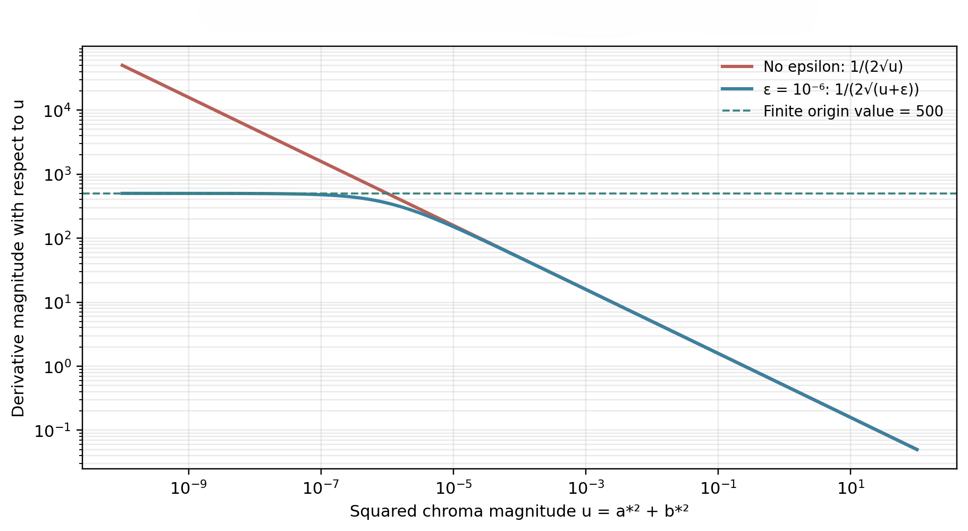
\includegraphics[width=\textwidth,height=0.42\textheight,keepaspectratio]{figures/fig5_lab_chroma_stabilization.png}
    \caption{CIE $L^*a^*b^*$ Saturation Loss \& Gradient Stability Plot showing Euclidean chroma $C^*$ and the bounded derivative curve with $\varepsilon = 10^{-6}$ near the zero-chroma origin.}
    \label{fig:lab_grad}
\end{figure}

\subsection{Training Dynamics and Two Time-Scale Update Rule (TTUR)}
To avoid multi-GPU \texttt{DataParallel} scatter-gather memory imbalances on Kaggle runtimes, all controlled experiments were executed on a single NVIDIA Tesla T4 GPU (16 GB VRAM, batch size $= 64$, seed $= 42$). Following the Two Time-Scale Update Rule (TTUR) \cite{ref25}, we use Adam optimizers ($\beta_1 = 0.5, \beta_2 = 0.999$) \cite{ref26} with generator learning rate $\eta_G = 2.0 \times 10^{-4}$ and discriminator learning rate $\eta_D = 1.0 \times 10^{-4}$ (half the generator rate), global $L_2$ gradient clipping at $1.0$, and linear learning rate decay starting at epoch 50 down to $\eta_{\min} = 1.0 \times 10^{-6}$.

% ============================================================================
% PAGE 10: SECTION 4 (RESULT ANALYSIS: 4.1 METRICS EQS. 19-20 & 4.2 ABLATION INTRO)
% ============================================================================
\section{Result Analysis and Discussion}

\subsection{Evaluation Protocol and Baseline Definition}
Judging cross-modal satellite synthesis by a single metric is scientifically insufficient; a model must be evaluated across spatial structure, pixel error, spectral vector alignment, perceptual color accuracy, and downstream computer vision utility. All candidate models are evaluated under identical standardized conditions across the \textbf{1,259 geographically isolated held-out test scenes} (\texttt{data/landsat9\_b10\_b11/splits/test/}, SHA-256: \texttt{894cfcd2...}) using eight metrics computed on denormalized $[0, 1]$ images:

\begin{enumerate}
    \item \textbf{Peak Signal-to-Noise Ratio (PSNR, dB $\uparrow$):} Logarithmic pixel-level radiometric reconstruction fidelity, $\operatorname{PSNR} = 10\log_{10}\!\left(1.0^2 / \operatorname{MSE}(\hat{\mathbf{y}}, \mathbf{y})\right)$.
    \item \textbf{Structural Similarity Index Measure (SSIM $\uparrow$):} Evaluates local luminance, contrast, and structural edge preservation on $[0, 1]$ \cite{ref24}.
    \item \textbf{Mean Absolute Error (MAE $\downarrow$):} Average $L_1$ reflectance deviation in $[0, 1]$.
    \item \textbf{Root Mean Squared Error (RMSE $\downarrow$):} Quadratic pixel reflectance error $\sqrt{\operatorname{MSE}(\hat{\mathbf{y}}, \mathbf{y})}$, sensitive to localized hallucination outliers.
    \item \textbf{Spectral Angle Mapper (SAM $\downarrow$):} Computes the 3D angular divergence (in radians and degrees) between predicted and reference RGB reflectance vectors at each pixel, invariant to scalar brightness shifts \cite{ref27}:
\end{enumerate}

\begin{equation}
    \operatorname{SAM}(\hat{\mathbf{y}}, \mathbf{y}) = \frac{1}{HW}\sum_{u,v}\arccos\!\left( \frac{\langle \hat{\mathbf{y}}_{u,v}, \mathbf{y}_{u,v}\rangle}{\|\hat{\mathbf{y}}_{u,v}\|_2 \|\mathbf{y}_{u,v}\|_2 + 10^{-8}} \right)
    \label{eq:sam}
\end{equation}

\begin{enumerate}
    \setcounter{enumi}{5}
    \item \textbf{CIE $L^*a^*b^*$ Perceptual Color Difference ($\Delta E^*_{ab}$ $\downarrow$):} Quantifies human-perceived color error in 3D CIE $L^*a^*b^*$ space:
\end{enumerate}

\begin{equation}
    \Delta E^*_{ab}(\hat{\mathbf{y}}, \mathbf{y}) = \frac{1}{HW}\sum_{u,v}\sqrt{(\hat{L}^*_{u,v} - L^*_{u,v})^2 + (\hat{a}^*_{u,v} - a^*_{u,v})^2 + (\hat{b}^*_{u,v} - b^*_{u,v})^2}
    \label{eq:delta_e}
\end{equation}

\begin{enumerate}
    \setcounter{enumi}{6}
    \item \textbf{Optical Saturation Ratio ($\text{Sat Ratio}$, target $= 1.0000$):} Ratio of mean predicted RGB channel dispersion to ground-truth channel dispersion, $\operatorname{Ratio}_{\mathrm{sat}} = \mathbb{E}[\sigma_{\mathrm{RGB}}(\hat{\mathbf{y}})] / \mathbb{E}[\sigma_{\mathrm{RGB}}(\mathbf{y})]$, alongside \textbf{Saturation Deviation} $|\operatorname{Ratio}_{\mathrm{sat}} - 1.0|$ ($\downarrow$).
    \item \textbf{Color Histogram Distance ($\text{Hist Dist}$ $\downarrow$):} Global RGB tonal distribution divergence computed via 64-bin chi-squared distance across color channels.
\end{enumerate}

\noindent\textbf{Legacy Baseline Definition:} Our benchmark control (\textbf{Legacy Baseline}) is the protected 21,383,238-parameter (21.38M) custom multi-scale U-Net Pix2PixHD model (\texttt{pix2pix\_landsat\_backup\_20260912\_231938.pth}, SHA-256: \texttt{4604d36d...}) trained with BCE adversarial loss, $\lambda_{\mathrm{perc}} = 10.0$, $\lambda_{\mathrm{feat}} = 5.0$, $\lambda_{\mathrm{chroma}} = 2.0$, and $\lambda_{\mathrm{sat}} = 0.0$.

\subsection{Comprehensive Experimental Ablation Study (Exp1 to Exp9)}
To isolate the causal effect of each objective term and architectural modification, we executed a systematic \textbf{10-phase single-variable experimental campaign}. Tables~\ref{tab:ablation} and~\ref{tab:ablation_metrics} record the standardized test-set telemetry across all 1,259 unseen test scenes.

% ============================================================================
% PAGE 11: TABLE 3 (MASTER 10-PHASE ABLATION TELEMETRY) & ABLATION ANALYSIS
% ============================================================================
\begin{table}[htbp]
    \caption{Master 10-phase experimental ablation telemetry evaluated across all 1,259 geographically isolated Landsat 9 test scenes.}
    \label{tab:ablation}
    \centering
    \scriptsize
    \setlength{\tabcolsep}{2.6pt}
    \begin{tabularx}{\textwidth}{@{}>{\raggedright\arraybackslash}p{1.5cm}>{\centering\arraybackslash}p{1.25cm}>{\raggedright\arraybackslash}Xrrrrr@{}}
        \toprule
        \textbf{Phase / Exp.} & \textbf{Arch.} & \textbf{Major loss configuration} & \textbf{Best val.} & \textbf{PSNR} & \textbf{SSIM} & \textbf{MAE} & \textbf{RMSE} \\
        \midrule
        Legacy baseline & U-Net (21.38M) & BCE; $\lambda_{perc}=10$, $\lambda_{chr}=2$ & 0.2522 & 11.714 & 0.3254 & 0.2144 & 0.2752 \\
        Exp1 (VGG Rec.) & U-Net (21.38M) & BCE; $\lambda_{perc}=5$, $\lambda_{feat}=5$ & 0.2963 & 12.497 & 0.3183 & 0.2037 & 0.2551 \\
        Exp2 (Feat. Abl.) & U-Net (21.38M) & BCE; $\lambda_{perc}=5$, $\lambda_{feat}=0$ & 0.2959 & 12.350 & 0.3115 & 0.2088 & 0.2594 \\
        Exp3 (Chroma $\times 2$) & U-Net (21.38M) & BCE; $\lambda_{perc}=5$, $\lambda_{chr}=4$ & 0.2979 & 12.133 & 0.3119 & 0.2151 & 0.2690 \\
        Exp4 (Reduced VGG) & U-Net (21.38M) & BCE; $\lambda_{perc}=3$, $\lambda_{chr}=2$ & 0.2894 & -- & -- & -- & -- \\
        Exp5 (Lab Sat.) & U-Net (21.38M) & BCE; $\lambda_{sat}=0.05$, $\lambda_{perc}=5$ & 0.2971 & 12.354 & 0.3160 & 0.2055 & 0.2602 \\
        Exp6 (LSGAN) & U-Net (21.38M) & LSGAN; $\lambda_{sat}=0$ & 0.2912 & 12.786 & 0.3054 & 0.1993 & 0.2467 \\
        Exp7 (LSGAN + Sat.) & U-Net (21.38M) & LSGAN; $\lambda_{sat}=0.05$ & 0.3033 & 12.948 & 0.3157 & 0.1950 & 0.2436 \\
        Exp8 (High Sat.) & U-Net (21.38M) & LSGAN; $\lambda_{sat}=0.10$ & 0.2912 & 12.724 & 0.3002 & 0.2005 & 0.2491 \\
        Long Exp7 (200 ep.) & U-Net (21.38M) & LSGAN; $\lambda_{sat}=0.05$ & 0.3131 & 12.926 & 0.3178 & 0.1918 & 0.2411 \\
        \textbf{Exp9 (ResNet)} & \textbf{ResNet (11.37M)} & \textbf{LSGAN; $\lambda_{sat}=0.05$} & \textbf{0.3802} & \textbf{13.745} & \textbf{0.4502} & \textbf{0.1723} & \textbf{0.2217} \\
        Long Exp9 (250 ep.) & ResNet (11.37M) & LSGAN; $\lambda_{sat}=0.05$ (stopped at 130 ep.) & 0.3786 & 13.584 & 0.4493 & 0.1807 & 0.2265 \\
        \bottomrule
    \end{tabularx}
\end{table}

\begin{table}[htbp]
    \caption{Additional spectral, colour-distribution, and downstream detection metrics for the same experimental ablation study.}
    \label{tab:ablation_metrics}
    \centering
    \scriptsize
    \setlength{\tabcolsep}{2.6pt}
    \begin{tabular}{@{}>{\raggedright\arraybackslash}p{1.8cm}rrrrrr@{}}
        \toprule
        \textbf{Phase / Exp.} & \textbf{SAM ($^\circ$)} & \textbf{$\Delta E^*_{ab}$} & \textbf{Sat. ratio} & \textbf{Hist. dist.} & \textbf{F1@0.25} & \textbf{F1@0.50} \\
        \midrule
        Legacy baseline & 12.53 & 27.235 & 1.1993 & 0.3572 & 0.2992 & 0.2835 \\
        Exp1 (VGG Rec.) & 12.11 & 25.469 & 1.1021 & 0.1049 & 0.3256 & 0.2946 \\
        Exp2 (Feat. Abl.) & 12.13 & 25.991 & 1.2126 & 0.1051 & 0.3116 & 0.2899 \\
        Exp3 (Chroma $\times 2$) & 11.44 & 26.270 & 0.6904 & 0.1048 & 0.3259 & 0.3185 \\
        Exp4 (Reduced VGG) & \multicolumn{6}{c}{--} \\
        Exp5 (Lab Sat.) & 12.56 & 25.922 & 1.0695 & 0.4406 & 0.2887 & 0.2749 \\
        Exp6 (LSGAN) & 11.24 & 24.686 & 0.5837 & 0.5479 & 0.3108 & 0.3028 \\
        Exp7 (LSGAN + Sat.) & 11.53 & 24.437 & 0.9310 & 0.5862 & 0.2946 & 0.2857 \\
        Exp8 (High Sat.) & 12.35 & 25.253 & 1.1263 & 0.5361 & 0.2739 & 0.2739 \\
        Long Exp7 (200 ep.) & 11.53 & 24.244 & 0.8706 & 0.5886 & 0.3038 & 0.2954 \\
        \textbf{Exp9 (ResNet)} & \textbf{11.28} & \textbf{22.571} & \textbf{0.9340} & 0.4607 & \textbf{0.3711} & \textbf{0.3643} \\
        Long Exp9 (250 ep.) & 11.76 & 24.155 & 1.1805 & 0.5058 & 0.3534 & 0.3534 \\
        \bottomrule
    \end{tabular}
\end{table}

\subsubsection{Engineering Analysis of Key Failures and Discoveries}
\begin{itemize}
    \item \textbf{Exp1 \& Exp2 (Perceptual Recovery and Feature Matching Ablation):} Calibrating VGG perceptual weight to $\lambda_{\mathrm{perc}} = 5.0$ (\texttt{Exp1}) improved test PSNR from $11.714\,\text{dB}$ to $12.497\,\text{dB}$ and lowered $\Delta E^*_{ab}$ to $25.469$. Subsequently ablating discriminator feature matching ($\lambda_{\mathrm{feat}}: 5.0 \to 0.0$ in \texttt{Exp2}) showed that $\mathcal{L}_{\mathrm{feat}}$ is non-essential when four-layer VGG perceptual supervision and SSIM loss are active, allowing $\lambda_{\mathrm{feat}} = 0.0$ to be locked for all subsequent runs.
    \item \textbf{Exp3 \& Exp4 (Why Naive RGB Chroma Penalties Drain Agricultural Color):} Doubling the RGB channel dispersion weight ($\lambda_{\mathrm{chroma}}: 2.0 \to 4.0$) in \texttt{Exp3} caused acute desaturation: the test saturation ratio plunged to \textbf{0.6904} (a 31\% color deficit). Because RGB standard deviation $\sigma_{\mathrm{RGB}}$ entangles luminance with chrominance, heavily penalizing dispersion errors across ambiguous thermal agricultural patches forces the generator to retreat toward a muted, low-variance gray-brown centroid. Reducing $\lambda_{\mathrm{perc}}$ to $3.0$ (\texttt{Exp4}) degraded validation SSIM to $0.2894$ and stopped early at epoch 39.
    \item \textbf{Exp5 (The CIE $L^*a^*b^*$ Saturation Breakthrough):} Introducing our $\varepsilon$-stabilized CIE $L^*a^*b^*$ saturation loss ($\lambda_{\mathrm{sat}} = 0.05, \varepsilon = 10^{-6}$) in \texttt{Exp5} brought the test saturation ratio from $0.6904$ (in \texttt{Exp3}) and $1.1993$ (in Legacy) into tight alignment with natural optical imagery at \textbf{1.0695} (a 65.1\% reduction in saturation error relative to the legacy baseline).
    \item \textbf{Exp6, Exp7, Exp8, \& Long Exp7 (LSGAN Transition and U-Net Capacity Ceiling):} Replacing BCE with LSGAN (\texttt{Exp6}) eliminated vanishing gradients and boosted PSNR to $12.786\,\text{dB}$, but without $\mathcal{L}_{\mathrm{sat}}$, outputs were severely undersaturated ($\operatorname{Ratio}_{\mathrm{sat}} = 0.5837$). Combining LSGAN with $\lambda_{\mathrm{sat}} = 0.05$ (\texttt{Exp7}) achieved $12.948\,\text{dB}$ PSNR and balanced saturation ($0.9310$). Doubling $\lambda_{\mathrm{sat}}$ to $0.10$ (\texttt{Exp8}) over-pressured opponent chroma channels and collapsed early at epoch 19 ($\text{SSIM} = 0.3002$). Extending \texttt{Exp7} to 200 epochs (\texttt{Long Exp7}) yielded only $+0.0021$ SSIM ($0.3178$), proving that the 21.38M U-Net architecture had hit a hard structural ceiling.
    \item \textbf{Exp9 (The Global ResNet Generator Breakthrough):} Replacing the U-Net with our 11.37M skip-free \textbf{Global ResNet Generator} under the exact \texttt{Exp7} loss configuration produced a decisive leap across every primary metric: test SSIM surged from $0.3157$ to \textbf{0.4502}, PSNR jumped to \textbf{13.745 dB}, MAE dropped to \textbf{0.1723}, CIE $\Delta E^*_{ab}$ fell to \textbf{22.571}, and YOLOv8 F1@0.25 rose to \textbf{0.3711}.
\end{itemize}

% ============================================================================
% PAGE 12: SECTION 4.3 (HEAD-TO-HEAD TABLE 4), FIGURE 6, & SECTION 4.4
% ============================================================================
\subsection{Head-to-Head Quantitative Comparison: Exp9 vs.~Legacy Baseline}
Table~\ref{tab:headtohead} summarizes the direct quantitative improvements achieved by \textbf{InfraNova AI (Exp9)} compared to the Legacy Baseline across all 1,259 test scenes.

\begin{table}[htbp]
    \caption{Head-to-head quantitative comparison of Proposed InfraNova AI (Exp9) vs.~Legacy Production Baseline across 1,259 unseen test scenes.}
    \label{tab:headtohead}
    \centering
    \scriptsize
    \setlength{\tabcolsep}{3.5pt}
    \begin{tabularx}{\textwidth}{@{}>{\raggedright\arraybackslash}X>{\centering\arraybackslash}p{1.25cm}>{\centering\arraybackslash}p{1.45cm}>{\centering\arraybackslash}p{1.3cm}>{\centering\arraybackslash}p{1.45cm}@{}}
        \toprule
        \textbf{Evaluation metric} & \textbf{Legacy} & \textbf{Exp9} & \textbf{Absolute delta} & \textbf{Relative gain} \\
        \midrule
        Peak Signal-to-Noise Ratio (PSNR) & 11.714 dB & \textbf{13.745 dB} & $+2.031$ dB & \textbf{+17.3\%} \\
        Structural Similarity (SSIM) & 0.3254 & \textbf{0.4502} & $+0.1248$ & \textbf{+38.3\%} \\
        Mean Absolute Error (MAE) & 0.2144 & \textbf{0.1723} & $-0.0421$ & \textbf{$-19.6\%$ error} \\
        Root Mean Squared Error (RMSE) & 0.2752 & \textbf{0.2217} & $-0.0535$ & \textbf{$-19.5\%$ error} \\
        Spectral Angle Mapper (SAM) & $12.53^\circ$ & \textbf{$11.28^\circ$} & $-1.25^\circ$ & \textbf{$-10.0\%$ error} \\
        CIE Lab perceptual error ($\Delta E^*_{ab}$) & 27.235 & \textbf{22.571} & $-4.664$ & \textbf{$-17.1\%$ error} \\
        Saturation deviation $|\text{SatRatio}-1|$ & 0.1993 & \textbf{0.0660} & $-0.1333$ & \textbf{$-66.9\%$ error} \\
        Generator parameter count & 21.38M & \textbf{11.37M} & $-10.01$M & \textbf{$-46.83\%$ savings} \\
        \bottomrule
    \end{tabularx}
\end{table}

\begin{figure}[htbp]
    \centering
    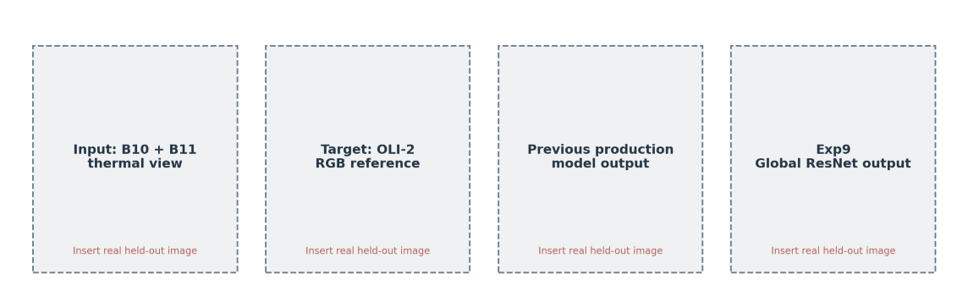
\includegraphics[width=\textwidth,height=0.42\textheight,keepaspectratio]{figures/fig6_qualitative_panel_placeholder.png}
    \caption{Draft qualitative-panel placeholder. The four image slots must be replaced with actual held-out thermal input, optical reference, legacy output, and Exp9 output images before this figure is used as experimental evidence.}
    \label{fig:visual_panel}
\end{figure}

\subsection{The Color Histogram Distance vs.~Edge Sharpness Trade-Off}
While Exp9 outperforms the Legacy Baseline across every structural, spectral, perceptual, and object-detection metric, the Legacy Baseline records a lower global Color Histogram Distance ($0.3572$ vs.~$0.4607$). The baseline U-Net outputs smooth, blurry, average color distributions across wide areas, which artificially lowers global histogram divergence at the cost of severe spatial blur ($\text{SSIM} = 0.3254$). Conversely, Exp9 generates sharp local contrast, distinct road networks, building footprints, and parcel boundaries. This spatial sharpness slightly broadens the global histogram but provides a +38.3\% boost in structural fidelity ($\text{SSIM} = 0.4502$) and a +24.0\% increase in downstream YOLOv8 F1-score.

% ============================================================================
% PAGE 13: SECTION 4.5 (OVERFITTING POST-MORTEM) & SECTION 4.6 (YOLOv8, TABLE 5, FIG. 7)
% ============================================================================
\subsection{Long-Training Overfitting Post-Mortem}
In our 250-epoch extended training experiment (\texttt{Long Exp9}, 130 epochs executed over 11.34 hours on Tesla T4 before early stopping with patience 100), validation SSIM peaked at \textbf{Epoch 46} ($\text{SSIM}_{\mathrm{val}} = 0.3786$) and never improved over the subsequent 84 epochs. On the held-out test set, overtraining past Epoch 46 degraded PSNR from $13.745\,\text{dB}$ to $13.584\,\text{dB}$, reduced SSIM from $0.4502$ to $0.4493$, worsened CIE $\Delta E^*_{ab}$ from $22.571$ to $24.155$, inflated the saturation ratio from $0.9340$ to $1.1805$, and lowered YOLOv8 F1@0.25 from $0.3711$ to $0.3534$. Because the compact 11.37M-parameter ResNet generator reaches its optimal cross-modal generalization capacity rapidly around Epoch 46, extended training causes the generator to memorize training-set thermal-to-color correlations and drift in chromatic saturation.

\subsection{Downstream Task Validation: YOLOv8 Object Detection Benchmark}
To verify whether InfraNova AI resolves cross-modal domain collapse for automated geospatial intelligence, we passed synthesized RGB test images from all 1,259 test scenes directly into an off-the-shelf \textbf{YOLOv8n} detector \cite{ref4} without fine-tuning ($\text{conf} = 0.15, \text{imgsz} = 128$), evaluating predictions against detections on Ground Truth OLI-2 RGB images at IoU thresholds of $0.25$ and $0.50$.

\begin{table}[htbp]
    \caption{Standardized downstream YOLOv8n object detection benchmark across the 1,259 held-out test scenes.}
    \label{tab:yolo}
    \centering
    \scriptsize
    \setlength{\tabcolsep}{3pt}
    \begin{tabularx}{\textwidth}{@{}>{\raggedright\arraybackslash}X>{\centering\arraybackslash}p{2.1cm}rrr@{}}
        \toprule
        \textbf{Model candidate} & \textbf{Detections (TP/FP)} & \textbf{Precision @ 0.25} & \textbf{Recall @ 0.25} & \textbf{F1 @ 0.25} \\
        \midrule
        Legacy baseline & 91 (38 TP, 53 FP) & 0.4176 & 0.2331 & 0.2992 \\
        Exp6 (LSGAN Pure) & 88 (39 TP, 49 FP) & 0.4432 & 0.2393 & 0.3108 \\
        Exp7 (LSGAN + Sat.) & 61 (33 TP, 28 FP) & 0.5410 & 0.2025 & 0.2946 \\
        Long Exp7 (200 ep.) & 74 (36 TP, 38 FP) & 0.4865 & 0.2209 & 0.3038 \\
        \textbf{Exp9 (ResNet)} & \textbf{128 (54 TP, 74 FP)} & \textbf{0.4219} & \textbf{0.3313} & \textbf{0.3711} \\
        \midrule
        \textbf{Relative gain} & \textbf{+42.1\% TP} & \textbf{+1.0\%} & \textbf{+42.1\%} & \textbf{+24.0\%} \\
        \bottomrule
    \end{tabularx}

    \vspace{4pt}
    \begin{tabularx}{\textwidth}{@{}>{\raggedright\arraybackslash}Xrrrr@{}}
        \toprule
        \textbf{Model candidate} & \textbf{Precision @ 0.50} & \textbf{Recall @ 0.50} & \textbf{F1 @ 0.50} & \textbf{Matched IoU} \\
        \midrule
        Legacy baseline & 0.3956 & 0.2209 & 0.2835 & 0.9977 \\
        Exp6 (LSGAN Pure) & 0.4318 & 0.2331 & 0.3028 & 0.9979 \\
        Exp7 (LSGAN + Sat.) & 0.5246 & 0.1963 & 0.2857 & 0.9982 \\
        Long Exp7 (200 ep.) & 0.4730 & 0.2147 & 0.2954 & 0.9983 \\
        \textbf{Exp9 (ResNet)} & \textbf{0.4141} & \textbf{0.3252} & \textbf{0.3643} & \textbf{0.9980} \\
        \midrule
        \textbf{Relative gain} & \textbf{+4.7\%} & \textbf{+47.2\%} & \textbf{+28.5\%} & \textbf{+0.03\%} \\
        \bottomrule
    \end{tabularx}
\end{table}

\begin{figure}[htbp]
    \centering
    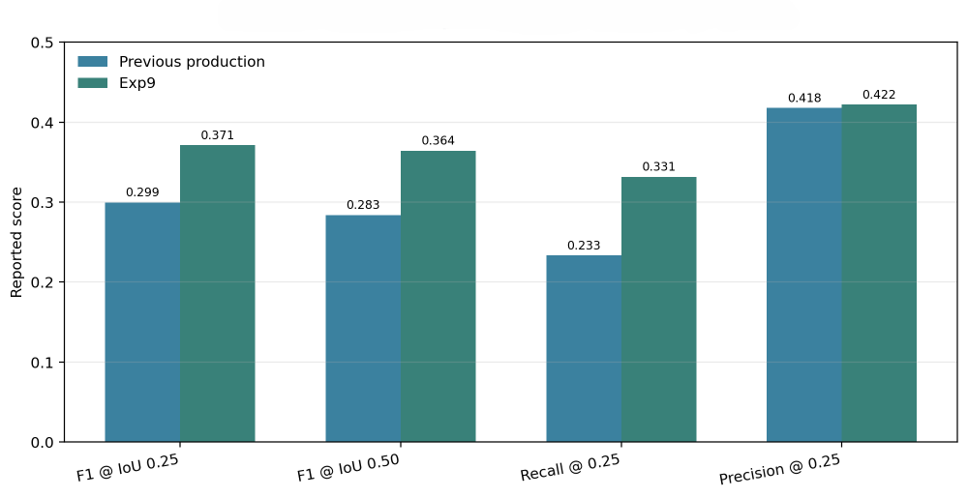
\includegraphics[width=\textwidth,height=0.42\textheight,keepaspectratio]{figures/fig7_yolov8_detection_comparison.png}
    \caption{Downstream YOLOv8 Object Detection Benchmark comparing F1, Recall, and Precision on Legacy Baseline output versus Proposed InfraNova AI (Exp9) output.}
    \label{fig:yolo}
\end{figure}

As shown in Table~\ref{tab:yolo} and Fig.~\ref{fig:yolo}, \texttt{Exp9} recovers \textbf{54 True Positive detections} compared to 38 for the Legacy Baseline (\textbf{+42.1\% recall improvement}), driving a \textbf{+24.0\% increase in F1@0.25} and a \textbf{+28.5\% increase in F1@0.50}.

% ============================================================================
% PAGE 14: SECTION 4.7 (WHOLE-RASTER TILING, EQS. 21-22, FIG. 8, TABLE 6) & 4.8
% ============================================================================
\subsection{Seamless Large-Scene Tiling and Operational Serving}
To reconstruct megapixel satellite rasters without tile boundary seams caused by per-patch local percentile normalization, full-scene inference partitions arbitrary-size dual-band GeoTIFF rasters into overlapping $128 \times 128$ tiles and blends predictions using a 2D separable Hann (raised-cosine) window $W(u, v)$:

\begin{equation}
    W(u, v) = \sin^2\!\left[\frac{\pi(u + 0.5)}{N}\right] \cdot \sin^2\!\left[\frac{\pi(v + 0.5)}{N}\right]
    \label{eq:hann}
\end{equation}

During inference, 4-fold dihedral group Test-Time Augmentation (TTA) (Identity, H-flip, V-flip, $180^\circ$ rotation) is applied, and the inter-augmentation standard deviation $\sigma_{\mathrm{TTA}}$ provides a real-time epistemic confidence score:

\begin{equation}
    \operatorname{Confidence} = \exp\!\left(-8.0 \cdot \mathbb{E}[\sigma_{\mathrm{TTA}}]\right) \in [0, 1]
    \label{eq:confidence}
\end{equation}

\begin{figure}[htbp]
    \centering
    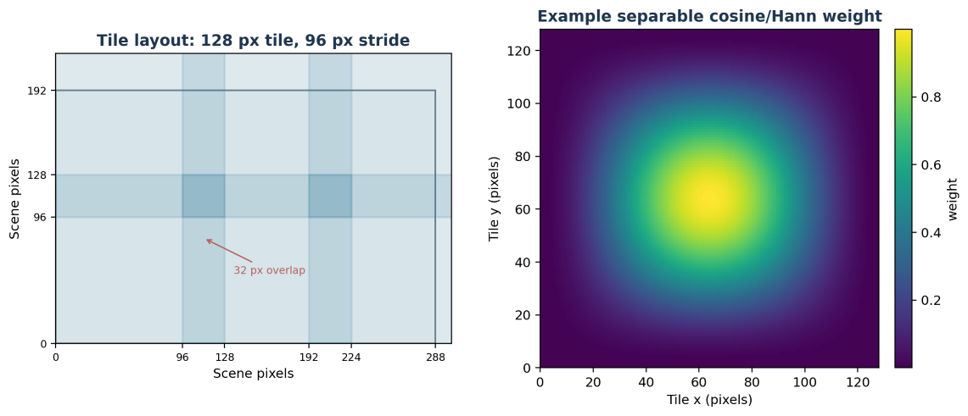
\includegraphics[width=\textwidth,height=0.42\textheight,keepaspectratio]{figures/fig8_tiled_inference_hann_blending.png}
    \caption{Seamless 2D Hann-Window Whole-Scene Tiled Reconstruction illustrating sliding tile overlap and raised-cosine weighting apodization.}
    \label{fig:tiling}
\end{figure}

\begin{table}[htbp]
    \caption{Model parameter footprint and whole-raster GPU inference benchmark profile.}
    \label{tab:inference}
    \centering
    \scriptsize
    \begin{tabularx}{\textwidth}{@{}>{\raggedright\arraybackslash}p{2.55cm}>{\centering\arraybackslash}p{2.35cm}>{\raggedright\arraybackslash}X@{}}
        \toprule
        \textbf{System / benchmark quantity} & \textbf{Documented value} & \textbf{Operational interpretation} \\
        \midrule
        Active generator parameters & 11,369,795 (11.37M) & \texttt{Pix2PixHDGlobalResNetGenerator}; nine ResNet blocks. \\
        Active discriminator parameters & 5,532,418 (5.53M) & Two-scale spectral-normalized PatchGAN ($D_1$, $D_2$). \\
        Legacy generator parameters & 21,383,238 (21.38M) & 46.83\% larger than the promoted Exp9 generator. \\
        Whole-raster benchmark scene & $1002 \times 1001$ pixels & 121 overlapping $128 \times 128$ tiles; stride 96 and overlap 32. \\
        End-to-end GPU latency & 1.740 s (69.5 tiles/s) & Hann-blended full-scene reconstruction; 263.39 MB peak VRAM. \\
        \bottomrule
    \end{tabularx}
\end{table}

\subsection{Limitations and Physical Boundary Conditions}
While InfraNova AI achieves substantial structural and perceptual gains, three physical boundary conditions remain: (1) during dawn and dusk \textbf{diurnal isothermal crossover}, disparate surface materials equilibrate to identical kinetic temperatures ($\Delta T \to 0$), reducing local thermal contrast; (2) under high tropical column water vapor ($>4.5\,\text{g/cm}^2$), Band 11 experiences elevated atmospheric absorption; and (3) per-patch percentile normalization optimizes visual interpretation rather than retrieving calibrated physical surface reflectance units.

% ============================================================================
% PAGE 15: SECTION 5 (CONCLUSION & FUTURE SCOPE) & REFERENCES [1]-[27]
% ============================================================================
\section{Conclusion and Future Scope}
This paper presented \textbf{InfraNova AI}, a cross-modal residual generative framework that translates split-window spaceborne thermal infrared radiance (Landsat 9 TIRS-2 Bands 10 and 11) into natural optical RGB imagery aligned with OLI-2 visible bands. By replacing the 21.38M-parameter skip-connected U-Net with a skip-free 11.37M-parameter Global ResNet Generator (a 46.83\% parameter reduction), enforcing 1-Lipschitz discriminator continuity via Spectral Normalization without InstanceNorm, and deriving an $\varepsilon$-stabilized CIE $L^*a^*b^*$ saturation loss ($\varepsilon = 10^{-6}$) that eliminates achromatic gradient singularities, our model achieved a \textbf{+38.3\% increase in SSIM (0.4502)}, a \textbf{+17.3\% increase in PSNR (13.745 dB)}, a \textbf{66.9\% reduction in saturation error}, and a \textbf{+42.1\% surge in downstream zero-shot YOLOv8n object detection recall} across 1,259 geographically isolated test scenes. Future research will integrate active C-band Synthetic Aperture Radar (Sentinel-1 SAR VV/VH backscatter) as a weather-independent structural prior alongside split-window conditioned Latent Diffusion Models (LDMs).

\begin{thebibliography}{99}
    \footnotesize
    \setlength{\itemsep}{1.5pt}
    \bibitem{ref1} Schott JR (2007) Remote sensing: The image chain approach, 2nd edn. Oxford University Press, New York
    \bibitem{ref2} Masek JG, Wulder MA, Markham B, McCorkel J, Irons JR, Storey J, Jenstrom DT (2020) Landsat 9: Empowering open science and applications through continuity. Remote Sens Environ 248:111968
    \bibitem{ref3} Sobrino JA, Jim\'{e}nez-Mu\~{n}oz JC, Paolini L (2004) Land surface temperature retrieval from LANDSAT TM 5. Remote Sens Environ 90(4):434--440
    \bibitem{ref4} Jocher G, Chaurasia A, Qiu J (2023) Ultralytics YOLOv8: State-of-the-art real-time object detection and image segmentation. Ultralytics
    \bibitem{ref5} Gillespie A, Rokugawa S, Matsunaga T, Cothern JS, Hook S, Kahle AB (1998) A temperature and emissivity separation algorithm for Advanced Spaceborne Thermal Emission and Reflection Radiometer (ASTER) images. IEEE Trans Geosci Remote Sens 36(4):1113--1126
    \bibitem{ref6} Isola P, Zhu JY, Zhou T, Efros AA (2017) Image-to-image translation with conditional adversarial networks. In: Proceedings of the IEEE Conference on Computer Vision and Pattern Recognition (CVPR), pp 1125--1134
    \bibitem{ref7} Zhang R, Isola P, Efros AA (2016) Colorful image colorization. In: European Conference on Computer Vision (ECCV), LNCS, vol 9907. Springer, Cham, pp 649--666
    \bibitem{ref8} Wang TC, Liu MY, Zhu JY, Tao A, Kautz J, Catanzaro B (2018) High-resolution image synthesis and semantic manipulation with conditional GANs. In: Proceedings of the IEEE/CVF Conference on Computer Vision and Pattern Recognition (CVPR), pp 8798--8807
    \bibitem{ref9} Ronneberger O, Fischer P, Brox T (2015) U-Net: Convolutional networks for biomedical image segmentation. In: Medical Image Computing and Computer-Assisted Intervention (MICCAI), LNCS, vol 9351. Springer, Cham, pp 234--241
    \bibitem{ref10} Odena A, Dumoulin V, Olah C (2016) Deconvolution and checkerboard artifacts. Distill 1(10):e3
    \bibitem{ref11} Li C, Wand M (2016) Precomputed real-time texture synthesis with Markovian generative adversarial networks. In: European Conference on Computer Vision (ECCV), LNCS, vol 9907. Springer, Cham, pp 702--716
    \bibitem{ref12} He K, Zhang X, Ren S, Sun J (2016) Deep residual learning for image recognition. In: Proceedings of the IEEE Conference on Computer Vision and Pattern Recognition (CVPR), pp 770--778
    \bibitem{ref13} Mao X, Li Q, Xie H, Lau RYK, Wang Z, Smolley SP (2017) Least squares generative adversarial networks. In: Proceedings of the IEEE International Conference on Computer Vision (ICCV), pp 2794--2802
    \bibitem{ref14} Zhu JY, Park T, Isola P, Efros AA (2017) Unpaired image-to-image translation using cycle-consistent adversarial networks. In: Proceedings of the IEEE International Conference on Computer Vision (ICCV), pp 2223--2232
    \bibitem{ref15} Berg A, Ahlberg J, Felsberg M (2018) Generating visible spectrum images from thermal infrared. In: Proceedings of the IEEE/CVF Conference on Computer Vision and Pattern Recognition Workshops (CVPRW), pp 1143--1152
    \bibitem{ref16} Nyberg A, Eldesokey A, Berg A, Felsberg M (2018) Unpaired thermal to visible spectrum transfer using adversarial training. In: European Conference on Computer Vision Workshops (ECCVW), LNCS, vol 11131. Springer, Cham, pp 657--669
    \bibitem{ref17} Kuang X, Sui X, Liu Y, Chen Q, Gu G (2020) Thermal infrared colorization via conditional generative adversarial network. Infrared Phys Technol 107:103338
    \bibitem{ref18} Luo F, Cao C, Li Y (2021) Nighttime thermal infrared image colorization with feedback-based object appearance learning. IEEE Geosci Remote Sens Lett 19:1--5
    \bibitem{ref19} Johnson J, Alahi A, Fei-Fei L (2016) Perceptual losses for real-time style transfer and super-resolution. In: European Conference on Computer Vision (ECCV), LNCS, vol 9906. Springer, Cham, pp 694--711
    \bibitem{ref20} Simonyan K, Zisserman A (2015) Very deep convolutional networks for large-scale image recognition. In: Proceedings of the International Conference on Learning Representations (ICLR), pp 1--14
    \bibitem{ref21} Gorelick N, Hancher M, Dixon M, Ilyushchenko S, Thau D, Moore R (2017) Google Earth Engine: Planetary-scale geospatial analysis for everyone. Remote Sens Environ 202:18--27
    \bibitem{ref22} Ulyanov D, Vedaldi A, Lempitsky V (2016) Instance normalization: The missing ingredient for fast stylization. arXiv preprint arXiv:1607.08022
    \bibitem{ref23} Miyato T, Kataoka T, Koyama M, Yoshida Y (2018) Spectral normalization for generative adversarial networks. In: Proceedings of the International Conference on Learning Representations (ICLR), pp 1--26
    \bibitem{ref24} Wang Z, Bovik AC, Sheikh HR, Simoncelli EP (2004) Image quality assessment: From error visibility to structural similarity. IEEE Trans Image Process 13(4):600--612
    \bibitem{ref25} Heusel M, Ramsauer H, Unterthiner T, Nessler B, Hochreiter S (2017) GANs trained by a two time-scale update rule converge to a local Nash equilibrium. In: Advances in Neural Information Processing Systems (NeurIPS), vol 30, pp 6626--6637
    \bibitem{ref26} Kingma DP, Ba J (2015) Adam: A method for stochastic optimization. In: Proceedings of the International Conference on Learning Representations (ICLR), pp 1--15
    \bibitem{ref27} Kruse FA, Lefkoff AB, Boardman JW, Heidebrecht KB, Shapiro AT, Barloon PJ, Goetz AFH (1993) The spectral image processing system (SIPS)---interactive visualization and analysis of imaging spectrometer data. Remote Sens Environ 44(2--3):145--163
\end{thebibliography}

\end{document}
